%!TEX root = slides.tex

\section{Marginal MCMC for Hierarchical Models}

\subsection{Background}
\begin{frame}{Joint MCMC}
	\begin{vfilleditems}
		\item In regular MCMC, we sample from the joint posterior of all the population and subject-specific parameters.
		\item Assume there are 3 subjects with subject parameters $\eta_1$, $\eta_2$ and $\eta_3$.
		\item Let the population parameters be $\theta$.
		\item Joint MCMC samples from the joint posterior:
		$$
			P(\theta, \eta_1, \eta_2, \eta_3 \mid \text{data})
		$$
		\item This means that the number of parameters to sample from increases linearly with the number of subjects.
	\end{vfilleditems}
\end{frame}

\begin{frame}{Marginal Posterior}
	\begin{vfilleditems}
		\item When there are many subjects and high correlation in the parameters in the posterior, the NUTS algorithm can often struggle to find good adaptation parameters.
		\item This is common if there are model identifiability issues and/or the priors are too weak compared to the likelihood.
		\item This is not uncommon in hierarchical models.
		\item After sampling from the joint posterior, we are often only interested in population parameters, e.g. to estimate a drug effect.
		\item The following is the marginal posterior of $\theta$ given the $\text{data}$.
		$$
			P(\theta \mid \text{data})
		$$
	\end{vfilleditems}
\end{frame}

\begin{frame}{Sample-Then-Marginalize vs Marginalize-Then-Sample}
	\begin{vfilleditems}
		\item There are 2 ways to marginalize out the subject-specific parameters:
		\begin{vfilleditems}
			\item Sample from the joint posterior and then ignore the subject-specific parameters. You can easily do this using \lstinline{BayesMCMC}.
			\item Integrate the subject-specific parameters out and then sample from the marginal posterior only. This is what \lstinline{MarginalMCMC} does in \lstinline{Pumas}.
		\end{vfilleditems}
		\item The marginal posterior probability is proportional to:
		$$
			P(\theta \mid \text{data}) \propto P(\theta, \text{data}) = \int_{\eta_3} \int_{\eta_2} \int_{\eta_1} P(\theta, \eta_1, \eta_2, \eta_3, \text{data}) d\eta_1 d\eta_2 d\eta_3
		$$
		\item MCMC can sample from $P(\theta \mid \text{data})$ given $P(\theta, \text{data})$ only without requiring the normalization constant.
	\end{vfilleditems}
\end{frame}

\subsection{Hierarchical Models}
\begin{frame}{Hierarchical Models}
	For hierarchical models, we can further break down the joint probability into the product of independent conditionals and $P(\theta)$:
	$$
		P(\theta, \eta_1, \eta_2, \eta_3, \text{data}) = P(\theta) \cdot \prod_{i=1}^3 P(\eta_i, \text{data}_i \mid \theta)
	$$
	where $\text{data}_i$ is the data of subject $i$.
\end{frame}

\begin{frame}{Hierarchical Models}
	The integral can therefore be simplified to the product of $P(\theta)$ and 3 smaller integrals:
	$$
		\begin{aligned}
			P(\theta, \text{data}) & = \int_{\eta_3} \int_{\eta_2} \int_{\eta_1} P(\theta) \cdot \prod_{i=1}^3 P(\eta_i, \text{data}_i \mid \theta) d\eta_1 d\eta_2 d\eta_3 \\
			                       & = P(\theta) \cdot \prod_{i=1}^3 \int_{\eta_i} P(\eta_i, \text{data}_i \mid \theta) d\eta_i
		\end{aligned}
	$$
	\vfill
	Each of the above smaller integrals has a low dimension.
\end{frame}

\begin{frame}{Approximate Marginalization}
	\begin{vfilleditems}
		\item The \lstinline{MarginalMCMC} algorithm in Pumas uses approximate integration methods, e.g. the Laplace method or the first order conditional estimation (FOCE) approximation of the Laplace method to compute the subject-specific integrals.
		\item This approximation is accurate if the conditional posterior $P(\eta_i | \theta, \text{data}_i)$ is approximately Gaussian.
		\item This is often the case if the model is conditionally identifiable wrt $\eta_i$ after fixing $\theta$ and there is enough data per subject to identify the true parameters $\eta_i$.
	\end{vfilleditems}
\end{frame}

\begin{frame}{Efficiency and Cost}
	\begin{vfilleditems}
		\item The remaining parameters $\theta$ are then sampled from their marginal posterior using the NUTS algorithm and a dense mass matrix.
		\item This tends to leads to better adaptation and more efficient sampling.
		\item However, each evaluation of $P(\theta, \text{data})$ requires solving as many optimization problems as the number of subjects which is significantly more expensive than evaluating the total joint probability.
	\end{vfilleditems}
\end{frame}

\begin{frame}{Efficiency and Cost}
	\begin{vfilleditems}
		\item So there is a tradeoff between the cost per HMC step (marginal MCMC is more expensive) and the number of steps per proposal (marginal MCMC requires less steps).
		\item However, the computational cost of marginal MCMC can be more effectively parallelized by parallelizing the subject integral computations.
		\item The computational effort per subject per HMC step in marginal MCMC is higher than the joint MCMC method.
		\item This makes up for the parallelism overhead of having to manage and communicate with multiple threads/processes.
	\end{vfilleditems}
\end{frame}

\subsection{Comparison to Joint MCMC}
\begin{frame}{Marginal vs Joint MCMC}
	\centering
	\small
	\begin{tabular}{|l|p{.3\textwidth}|p{.3\textwidth}|}
		\toprule
		                              & \textcolor{blue}{\textbf{Marginal MCMC}}                                                                                  & \textcolor{red}{\textbf{Joint MCMC}} \\ \midrule
		\textbf{Number of parameters} & Low                                                                                                                       & High                                 \\ \midrule
		\textbf{Accuracy}             & Approximate even for infinite samples unless the conditional posterior $P(\eta_i \mid \theta, \text{data}_i)$ is Gaussian & Exact with infinite samples          \\ \midrule
		\textbf{Cost per HMC step}    & High                                                                                                                      & Low                                  \\ \midrule
		\textbf{Mass matrix}          & Dense                                                                                                                     & Diagonal (by default)                \\ \midrule
		\textbf{Max tree depth}       & Often low                                                                                                                 & Often high                           \\ \midrule
		\textbf{Parallelism}          & Efficient for all models                                                                                                  & Efficient only for difficult models  \\
		\bottomrule
	\end{tabular}
\end{frame}

\begin{frame}{Example: Rare Disease Modelling}
	\begin{vfilleditems}
		\item \textbf{Question}: Can we use prior information to reduce the number of subjects needed in a rare diseases study?
		\item \textbf{Experiment}:
		\begin{vfilleditems}
			\item Given a drug model for a rare disease with long-term disease progression effects and short-term symptomatic effects.
			\item Simulate 2 population arms in a study – placebo and treatment (trt = 0/1).
			\item Simulate clinical outcomes for each arm under the assumption that the drug has both long- and short-term effects.
			\item Run frequentist and Bayesian analysis to infer the drug effects given the synthetic data.
			\item Identify confidence and credible intervals for parameters.
		\end{vfilleditems}
	\end{vfilleditems}
\end{frame}

\begin{frame}{Example: Rare Disease Modelling}
	\centering
	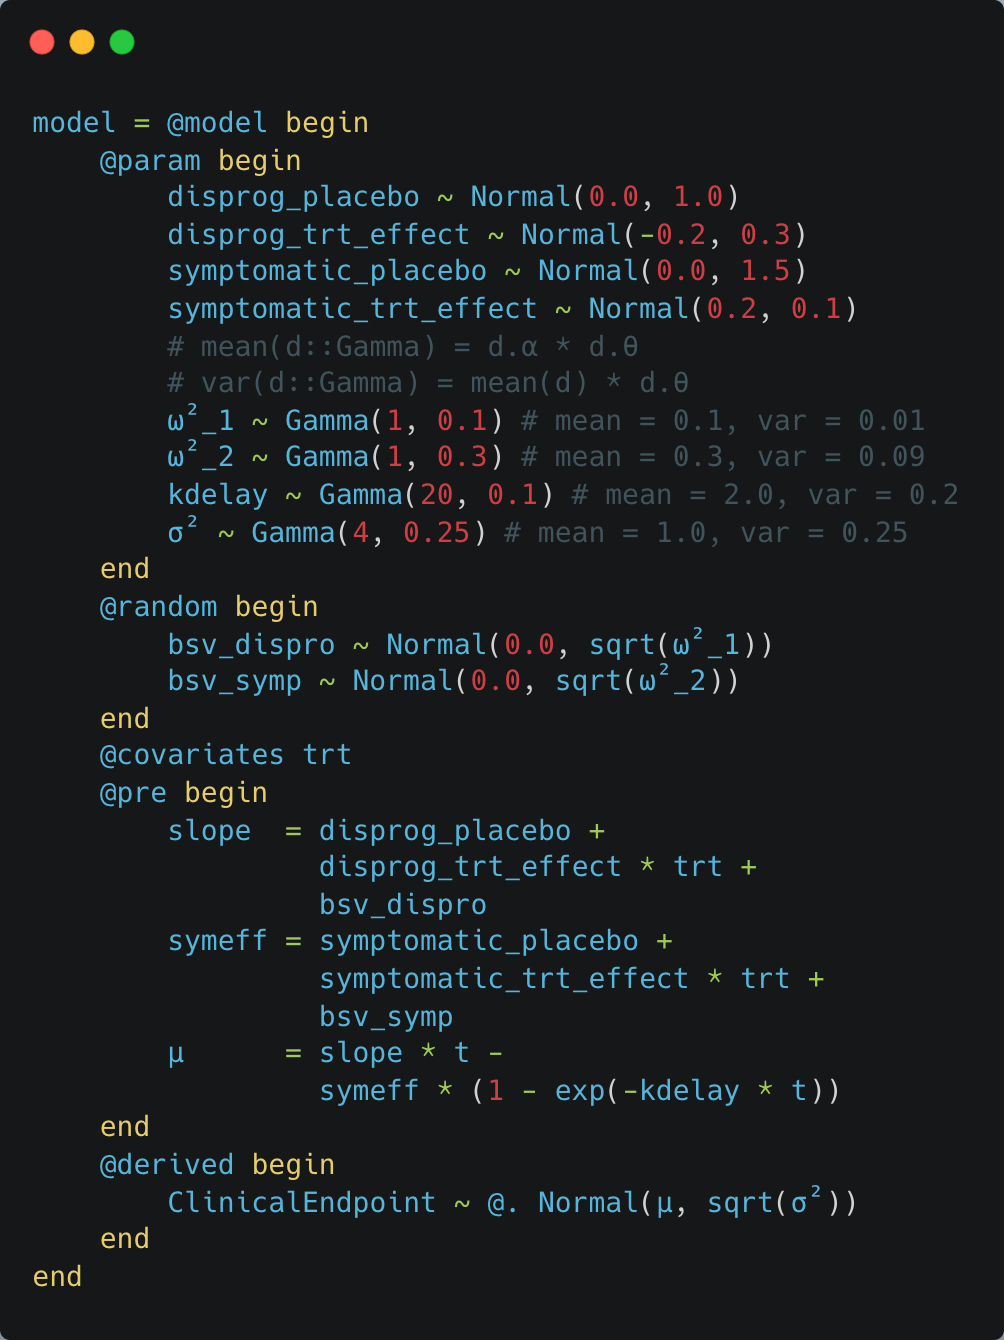
\includegraphics[width=0.35\columnwidth]{rare_disease.png}
\end{frame}

\begin{frame}{Example: Rare Disease Modelling}
	\begin{columns}
		\begin{column}{0.5\textwidth}
			\centering
			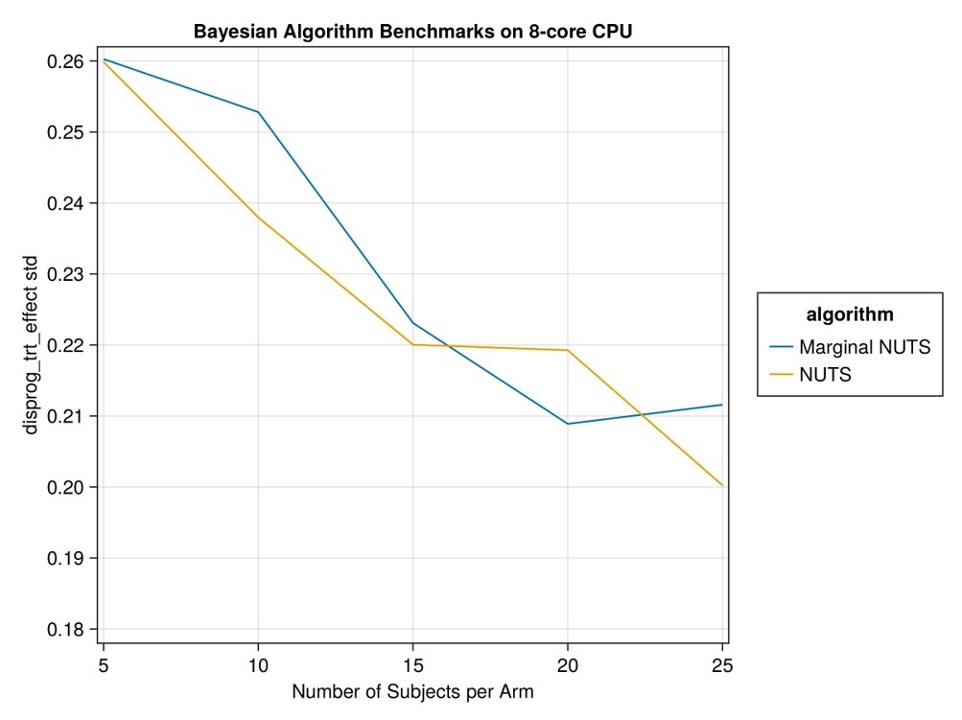
\includegraphics[width=\columnwidth]{marginal_mcmc_1.jpg}
		\end{column}
		\begin{column}{0.5\textwidth}
			\centering
			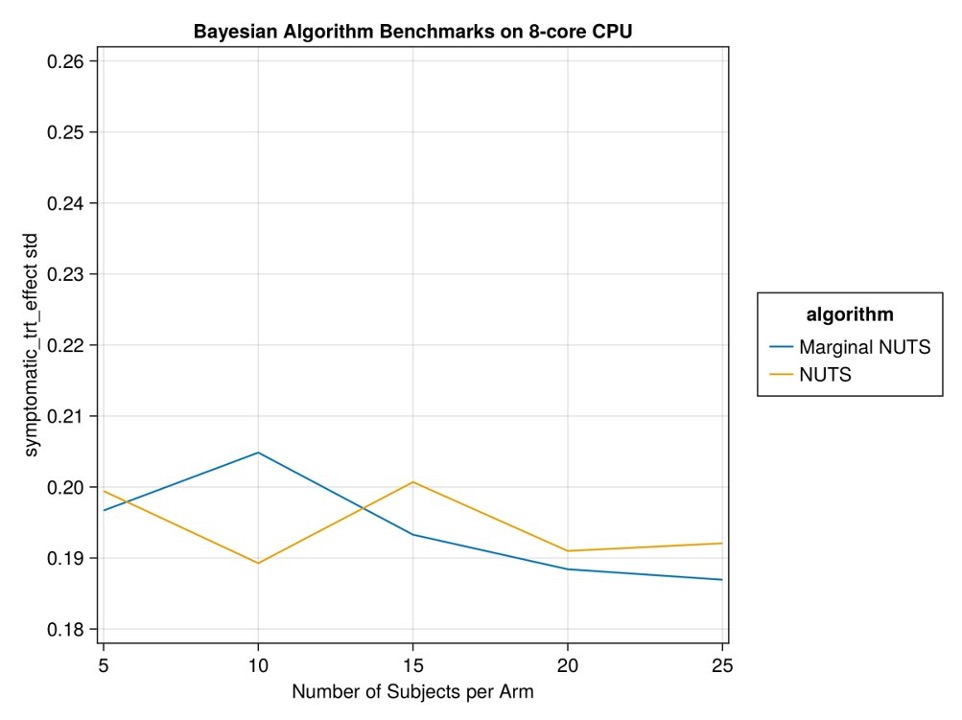
\includegraphics[width=\columnwidth]{marginal_mcmc_2.jpg}
		\end{column}
	\end{columns}
\end{frame}

\begin{frame}{Example: Rare Disease Modelling}
	\begin{columns}
		\begin{column}{0.5\textwidth}
			\centering
			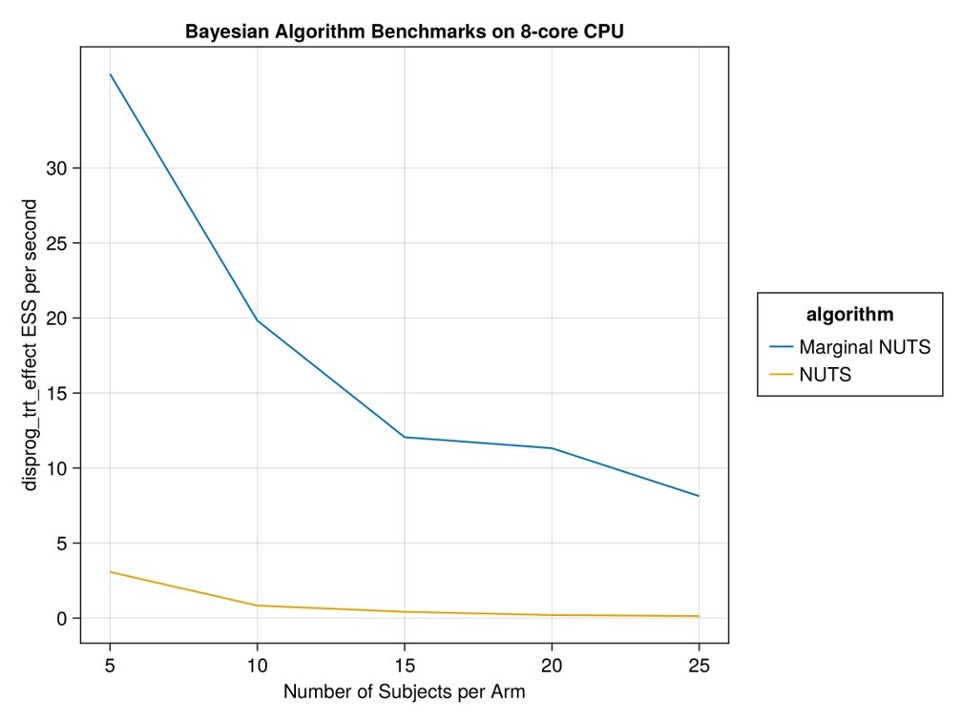
\includegraphics[width=\columnwidth]{marginal_mcmc_3.jpg}
		\end{column}
		\begin{column}{0.5\textwidth}
			\centering
			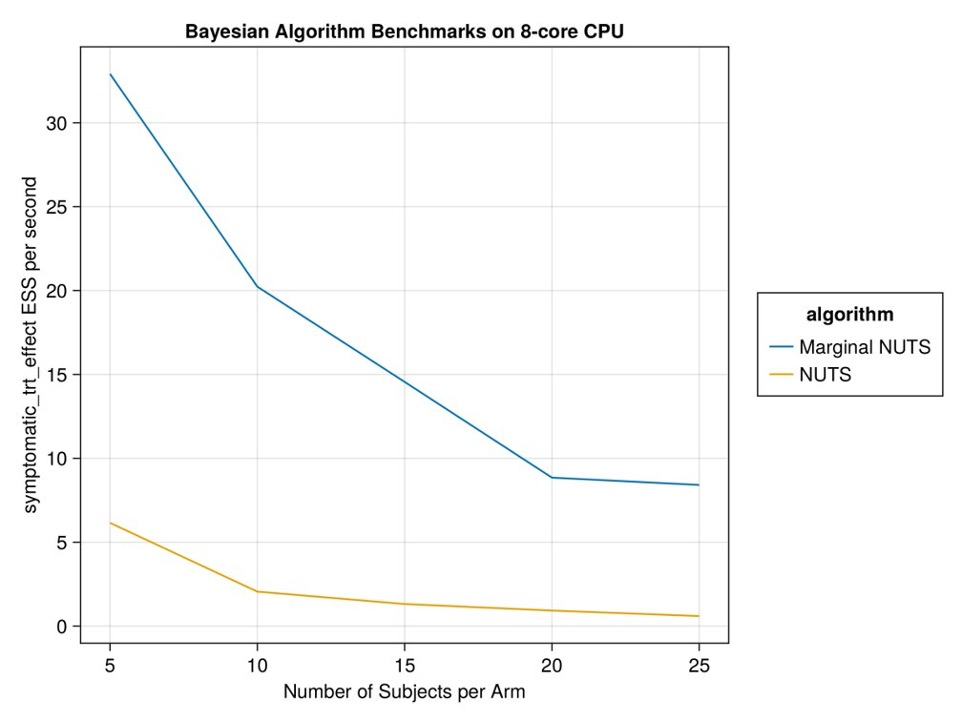
\includegraphics[width=\columnwidth]{marginal_mcmc_4.jpg}
		\end{column}
	\end{columns}
\end{frame}

\begin{frame}{Example: Rare Disease Modelling}
	\begin{columns}
		\begin{column}{0.5\textwidth}
			\centering
			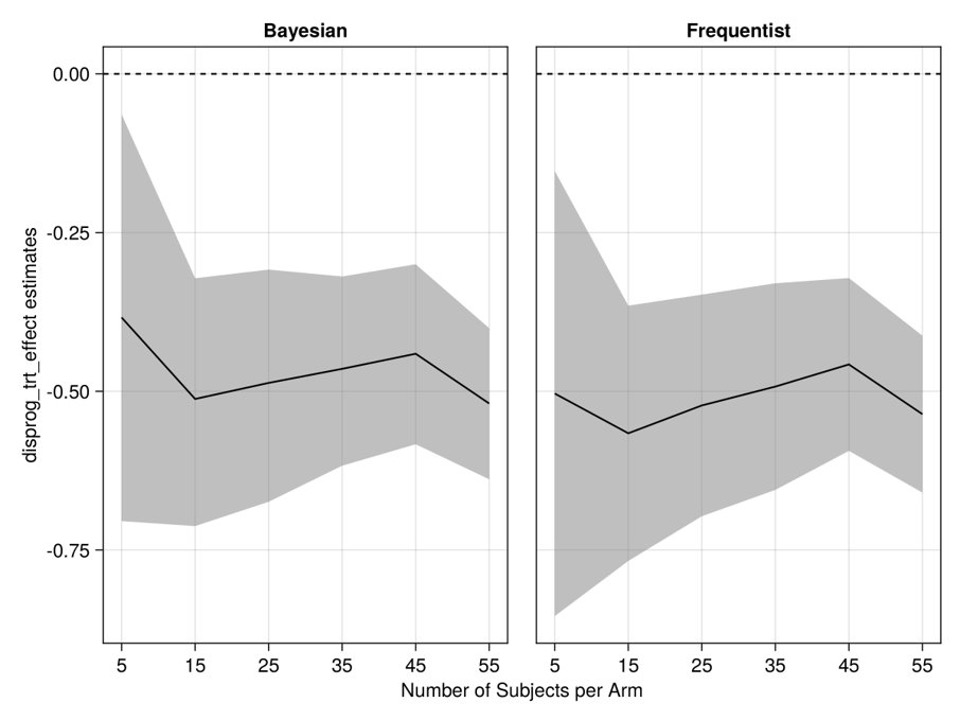
\includegraphics[width=\columnwidth]{rare_disease_intervals_1.jpg}
		\end{column}
		\begin{column}{0.5\textwidth}
			\centering
			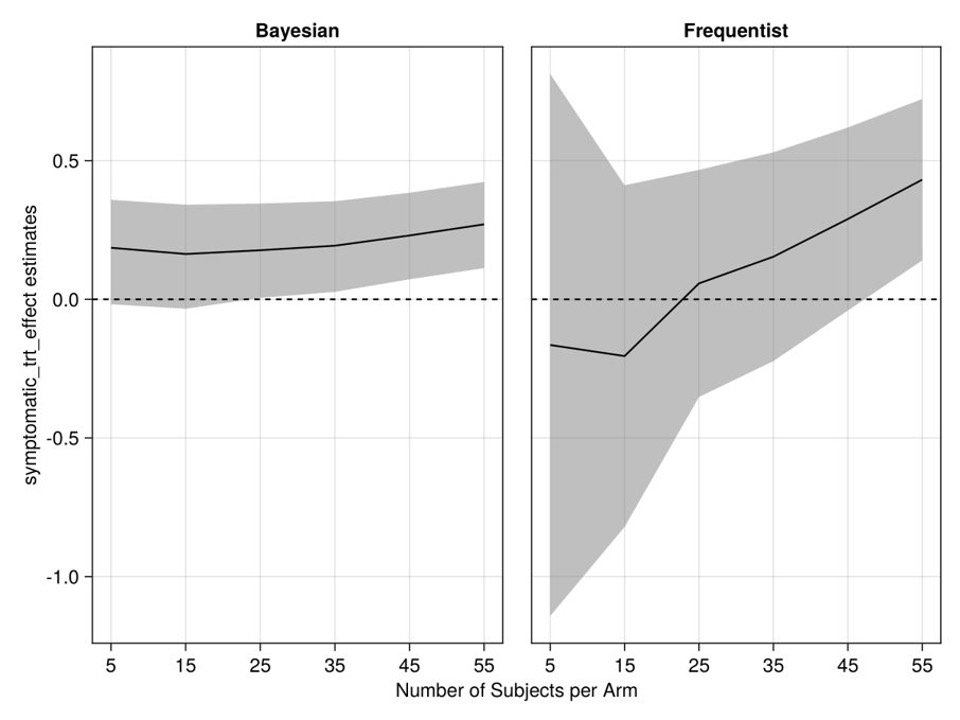
\includegraphics[width=\columnwidth]{rare_disease_intervals_2.jpg}
		\end{column}
	\end{columns}
\end{frame}
